\section{Decibilidad, semidecibilidad y computabilidad}
\subsection{Equivalencia entre TM y programas}
\subsubsection{\textit{k}-máquina de Turing}
\begin{easylist}[itemize]
& En esta sección veremos que las TM son tan expresivas como cualquiera de los lenguajes de programación que usamos habitualmente.

& Una extensión de las máquinas de Turing consiste en añadir una cinta con su propio cabezal. Son las 2-TM. Como veremos luego, esta ganancia en capacidad no permite reconocer más lenguajes.

& La explicamos mediante un ejemplo. Vimos ya una máquina de Turing para el lenguaje $\{w\#w \colon w\in\{0,1\}^*\}$. Veremos que, con dos cintas, la construcción del autómata se simplifica.

& Para la máquina de Turing con dos cintas asumimos que, inicialmente, la entrada se halla en la primera cinta y que la segunda cinta no contiene información. También asumimos que ambos cabezales apuntan a las respectivas posiciones 1. 

$\vartriangleright \; 0 \; 1 \; 1 \; \dots \; \# \; 0 \; 1 \; 1 \; \dots\;  \blanco \;  \blanco\; \dots$

$\vartriangleright \;  \blanco\;  \blanco \; \dots$

& La idea será copiar la palabra a la izquierda del separador sobre la segunda cinta y, a continuación, compararla directamente con la palabra que se encuentra a la derecha del separador.

$\vartriangleright \; 0 \; 1 \; 1 \; \dots \; \# \; 0 \; 1 \; 1 \; \dots\; \blanco \;  \blanco \; \dots$

$\vartriangleright 0 \; 1 \; 1 \; \dots \;  \blanco \;  \blanco \; \dots$

& Este es el grafo de estados.

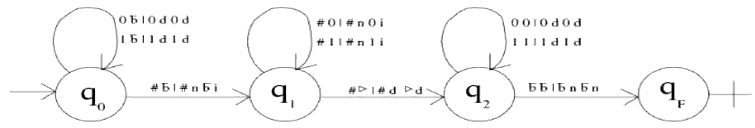
\includegraphics[width=0.8\textwidth]{t8-1.png}

&  Nótese que, ahora, las transiciones están etiquetadas con más información. La parte de la condición tiene ahora el símbolo que hay que leer de la primera cinta y el que hay de leer de la segunda cinta. En la acción indicamos qué símbolo hay que escribir en la primera cinta y adónde mover el cabezal de la primera cinta, y qué símbolo hay que escribir en la segunda cinta y adónde mover el cabezal de la segunda cinta.

& Explicación de la TM:
&& Inicialmente (en $q_0$), copiamos el contenido de la primera cinta en la segunda.

&& Al llegar al separador, pasamos a $q_1$ y regresamos el cabezal de la segunda cinta hasta el principio.

&& A continuación, iniciamos el proceso de comparar ambas palabras en $q_2$. Si la comparación termina satisfactoriamente, vamos a estado aceptador.

& El programa es más sencillo ahora, ya que disponemos de más capacidades. Sin embargo, toda 2-TM se puede simular con una sola TM.

& La idea que usamos es la siguiente: podemos representar el contenido de dos cintas mediante una sola cinta usando un símbolo adicional (\$) para separar ambos contenidos. Uno de los símbolos de la primera cinta quedará marcado de manera especial para recordar que ahí se encuentra el cabezal. Similarmente, uno de los símbolos de la segunda cinta quedará marcado de forma especial para recordar que ahí se encuentra el cabezal (aquí, $a'$ y $b'$).

& Es decir, $\vartriangleright a b \dots b b' a \dots b a \$ b a  \dots b a' a \dots a a \blanco \blanco \blanco \dots$.

& Para simular una transición de la 2-TM, nos veremos obligados a recorrer toda la palabra para ver cuáles son los símbolos apuntados por los cabezales. A continuación, deberemos pasar por ambos cabezales para actualizarlos convenientemente.

& Adicionalmente, puede ocurrir que tengamos que aumentar el tamaño de la palabra izquierda porque estamos accediendo a los blancos del final. Esto nos obligará a \textit{shiftar} la palabra derecha a posiciones más a la derecha.

& Esta idea se puede extender a $k$-TM con más cintas.

\end{easylist}

\subsubsection{Lenguajes de programación}
\begin{easylist}[itemize]

& Pasamos ahora a hablar de lenguajes de programación de más alto nivel.

& Los compiladores convierten lenguajes de programación a lenguajes de bajo nivel de ensamblador dependientes de la arquitectura.

& Estos usan un número limitado de registros ($R_1, \dots, R_n$) y una memoria de forma indexada: $M[0]$, $M[1]$, ...

& Las instruciones son del tipo:

\begin{lstlisting}
    $R_1$ := $R_2$ + $R_3$
    If $R_1$ = 0 Goto Etiqueta
    $R_1$ := $M$[35]
    $M$[13] := $R_5$
    $M$[$R_1$] := $R_2$
    $R_2$ := $M$[$R_1$]
\end{lstlisting}

& Puestos a asumir que trabajamos con memoria infinita, supondremos que, aun cuando contamos con un número finito de registros, la memoria es infinita y que, de hecho, cada registro y cada posición de memoria puede guardar, por ejemplo, un número natural arbitrariamente grande.

& En tal caso, son imprescindibles las instrucciones que involucran acceso indirecto como $M[R_1] \leftarrow R_2$ o $R_2 \leftarrow M[R_1]$, pues si solo pudiésemos acceder solo del modo $M[13] \leftarrow R_5$, solo podríamos acceder a las posiciones de memoria marcadas explícitamente en nuestro programa, y este consta de un número finito de instrucciones.

& Con una máquina de Turing con varias cintas, podemos representar el contenido de cada registro en una cinta distinta. Además, podemos guardar el contenido de toda la memoria en una cinta adicional usando separadores adecuadamente para delimitar el contenido de cada posición que haya sido accedida en algún momento de una ejecución.

& Veremos la instrucción $R_2 \leftarrow M[R_1]$.

& Para simplificar, suponemos que tenemos 3 cintas. La primera representa el contenido $x$ de $R_1$; la segunda, el contenido de $R_2$ que inicialmente está vacía, la tercera representa la memoria con registros guardando palabras sobre 0s y 1s separadas por el símbolo \#.

& Además, asumiremos que, inicialmente, el cabezal de la primera cinta se encuentra al final de $x$, el de la segunda apunta al primer blanco, y el de la tercera apunta al primer separador.

$\vartriangleright\; \dots \; x \; \dots \;  \blanco \;  \blanco\dots$

$\vartriangleright\;  \blanco\;  \blanco\; \dots$

$\vartriangleright\; \#\; w_0 \; \# \; w_1 \; \# \; \dots \; \# \; w_k \;  \blanco \;  \blanco\; \dots$

& La idea será ir avanzando por la memoria al tiempo que restamos 1 unidad al valor de la primera cinta cada vez que pasamos de largo un nuevo separador. En el momento en que la primera cinta ha llegado a 0, sabemos que estamos apuntando a la posición indexada por $x$. Entonces, procederemos a copiar el contenido sobre la segunda cinta.

& El fragmento de grafo de estados es el siguiente.\footnote{Consultad \url{http://youtu.be/fQltYKdFr1E} a partir del minuto 7:25 para ver una descripción del autómata.}

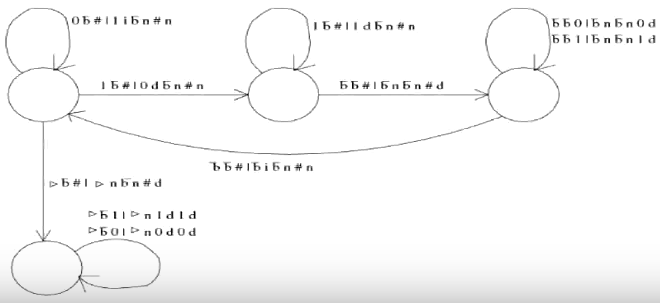
\includegraphics[width=0.8\textwidth]{t8-2.png}

\end{easylist}



\subsection{Asunciones sobre TM y programas}
\subsubsection{Primera asunción}
\begin{easylist}[itemize]
& Consideramos máquina de Turing y programa como sinónimos. Ya hemos justificado anteriormente que las máquinas de Turing pueden simular a cualquier lenguaje de programación; por tanto, nos permitiremos describir procesos en un lenguaje de alto nivel dando por sentado que tenemos su equivalente en TM o que de hecho eso ya es una TM.

& Por ejemplo, este programa es una TM que acepta cualquier entrada:

\begin{lstlisting}
Entrada $x$
       Aceptar
\end{lstlisting}

& Este otro es una TM que, dada una palabra de entrada que codifica un número natural, llega a estado aceptador dejando como resultado en la cinta la codificación del natural resultante de multiplicar por $2$ el que teníamos en la entrada.

\begin{lstlisting}
Entrada $x$
       Salida 2 * $x$
\end{lstlisting}


& Finalmente, este es un programa que decide el lenguaje $\{w \# w\colon w \in\{0,1\}^*\}$.

\begin{lstlisting}
Entrada $w$
    Si $w$ es de la forma $w'\#w'$ entonces Aceptar
    Si no Rechazar
\end{lstlisting}

& Recordemos que este lenguaje concreto ya habíamos visto una TM que lo reconocía.

& Nótese que \verb|Rechazar| corresponde a que la máquina para habiendo llegado a una configuración no aceptadora desde la que no hay transición definida.

\end{easylist}

\subsubsection{Segunda asunción}
\begin{easylist}[itemize]
& Todas las entradas se codifican con números naturales. Los resultados también son números naturales.

& Esto es porque las máquinas codifican toda la información con $0$s y $1$s. Por tanto, es creíble que las entradas y salidas de una máquina se puedan codificar mediante naturales.

& Ejemplos:
&& Entrada $w$ donde $w$ es una palabra. Cuando nos convenga, podremos asumir que recibimos un número natural que codifica una palabra.

&& Entrada $\langle x, y\rangle$. Es decir, una pareja de naturales. También podremos asumir que recibe un natural que codifica una palabra de naturales.

&& También se pueden representar una CFG $G$, un DFA $A$ o una terna con dos palabras y un sistema de reescritura: $\langle u, v, R = \{u_1 \to v_1, \dots, u_n \to v_n\}\rangle$.

\end{easylist}

\subsubsection{Tercera asunción}
\begin{easylist}[itemize]
& Cuando nos convenga, asumiremos que nuestro sistema de codificación enumera todas las entradas correctas.

& Por ejemplo, el conjunto de todos los DFA que son mínimos. Lo podemos ver como un conjunto de naturales que codifican DFA. En general, el complementario de este conjunto contendría: por un lado, a los naturales que codifican DFA no mínimos y a los naturales que no codifican correctamente ningún DFA.

& Si asumimos que el sistema de codificación asocia a cada natural un DFA de manera biunívoca, entonces el complementario es el que aparece a la derecha de la igualdad. $\{A \in \textrm{DFA} \colon A \textrm{ es mínimo}\} = \overline{\{A \in \textrm{DFA}\colon A \textrm{ no es mínimo}\}}$.

& Lo mismo sucede para ternas $\langle u, v, R\rangle$.

\end{easylist}


\subsubsection{Cuarta asunción}
\begin{easylist}[itemize]
& El conjunto de todos los programas se puede enumerar mediante los números naturales, ya que nuestros programas quedan almacenados mediante $0$s y $1$s. Asumimos una codificación fija concreta, sin especificar cuál; pues es irrelevante cuál sea mediante enumere a todos los programas posibles y sea codificable y descodificable algorítmicamente.

& Bajo esta suposición, mediante $M_n$ denotaremos a la máquina codificada por el número natural $n$.

& Esto puede ocasionar ambigüedad, pues $M_1$ significará la máquina $1$ o bien la máquina codificada por 1. El contexto soluciona esta ambigüedad.

\end{easylist}


\subsubsection{Quinta asunción}
\begin{easylist}[itemize]
& Podemos ejecutar programas desde otros programas. Es decir, existe un intérprete $U$ capaz de simular la ejecución de otro programa con una cierta entrada. Esta asunción es natural, pues se trata de la idea básica de los intérpretes y compiladores.

& Por ejemplo, este programa recibe un natural que codifica a dos naturales $\langle x, y\rangle$, simula la ejecución del programa codificado por $x$ con entrada $y$ y da como salida la misma salida de dicha ejecución. Esta no es más que una posible implementación de la máquina universal usando una instrucción que, de hecho, asume ya otra implementación de la máquina universal. Por supuesto, esta máquina se queda colgada con una entrada si esta ejecución no para.

$U(\langle x, y\rangle) = M_x(y)$

\begin{lstlisting}
Entrada $\langle x, y \rangle$
       Salida $M_x(y)$
\end{lstlisting}

& En este otro ejemplo ejecutamos el intérprete solo durante 100 pasos. Así, podemos ejecutar un intérprete por tiempo limitado. Podemos asumir que, con un paso, nos referimos a una transición de la TM.

\begin{lstlisting}
Entrada $\langle x, y \rangle$
       Si $M_x(y)$ para en 100 pasos, entonces Salida $M_x (y)$
       Si no, entonces Salida 0
\end{lstlisting}

& Para cada número natural $n$, con $\varphi_n$ denotamos la función computada por la máquina codificada por $n$: $\varphi_n \equiv \varphi_{M_n}$; y con $\mathcal L_n$, denotamos el lenguaje aceptado por la máquina codificada por $n$: $\mathcal L_n = \mathcal L(M_n)$.

& Nótese que, cuando la función computada por $n$ está definida para un cierto $m$ (esto es, $\varphi_n(m) \downarrow$), la máquina codificada por $n$ con entrada $m$ da el mismo resultado: $\varphi_n(m) = M_n(m)$.

& Pero, recuérdese que, aun cuando la función no esté definida, la máquina puede parar llegando a una configuración terminal no aceptadora ($\varphi_n(m) \uparrow$ o $M_n(m)  \downarrow$).

& De hecho, $M_n$ y $\varphi_n$ son objetos muy distintos.

& Por ejemplo, sea $n$ el número que codifica el programa

\begin{lstlisting}
Entrada $x$
    Salida 2 * $x$
\end{lstlisting}

& Tenemos que $M_n$ es justamente el programa (el bloque de código); en cambio, $\varphi_n$ es la función que implementa. Es decir: $M_n \neq \varphi_n = \{(0,0), (1,2), (2,4), \dots\}$.

& En el caso en que $n$ codifique a un programa que para siempre y rechaza o a un programa que no para con ninguna entrada, $\varphi_n$ es el conjunto vacío ($M_n \neq \varphi_n = \varnothing$) también llamada \textit{función vacía} o \textit{totalmente indefinida}.

\begin{lstlisting}
Entrada $x$
       Rechazar
\end{lstlisting}

\begin{lstlisting}
Entrada $x$
       Colgarse
\end{lstlisting}

& Podemos ahora redefinir nociones que ya habíamos introducido.

& Un subconjunto $C \subseteq N$ de los naturales es decible si existe un natural tal que la máquina que codifica lo reconoce y para con toda entrada: $C \in \textrm{Dec} \equiv \exists x \colon (\textrm{Dom}(\varphi_x) = C \land \forall y \colon M_x(y) \downarrow)$.

& Un subconjunto $C \subseteq N$ de los naturales es semi-decible si existe un natural tal que la máquina que lo codifica lo reconoce: $C \in \textrm{semi-Dec} \equiv \exists x \colon \mathcal L_x = C$.

& Una función es computable si existe un natural tal que, la máquina que lo codifica, la computa: si $f \colon \mathbb N \to \mathbb N$, entonces $f$ es computable si $\exists x \colon \varphi_x = f$.

\end{easylist}

\subsection{Operaciones sobre TM y programas}
\textit{Falta redactarlo}
\begin{easylist}[itemize]
\end{easylist}